\subsection{Overview} 
\label{ssec:overview}
A schematic overview of the sensor is shown in \cref{tkz:schematic_overview}.

\begin{figure}[H]
    \centering



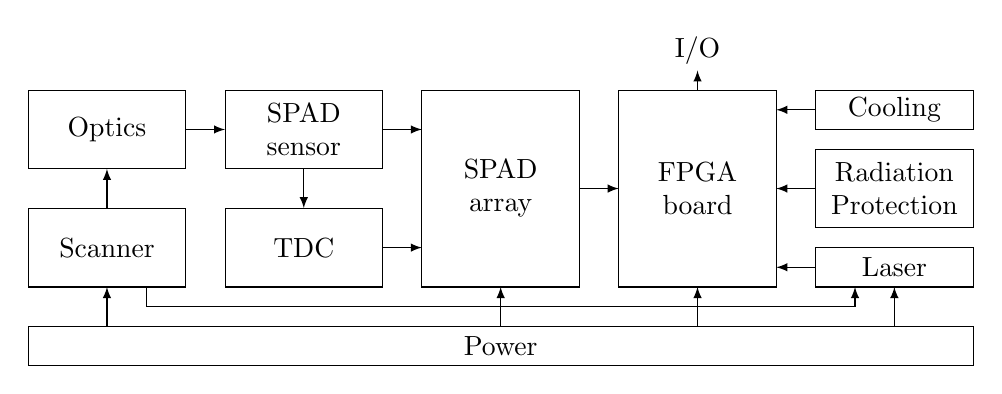
\begin{tikzpicture}[scale=.5]

\draw  (13,2) rectangle (17,1) node[pos=.5, align=center]{Cooling};
\draw  (13,0.5) rectangle (17,-1.5) node[pos=.5, align=center]{Radiation\\Protection};
\draw  (-7,-4) rectangle (17,-5) node[pos=.5, align=center]{Power};
\draw  (13,-2) rectangle (17,-3) node[pos=.5, align=center]{Laser};
\draw  (8,2) rectangle (12,-3) node[pos=.5, align=center]{FPGA\\board};
\draw  (3,2) rectangle (7,-3) node[pos=.5, align=center]{SPAD\\array};
\draw  (-2,2) rectangle (2,0) node[pos=.5, align=center]{SPAD\\sensor};
\draw  (-7,2) rectangle (-3,0) node[pos=.5, align=center]{Optics};
\draw  (-7,-1) rectangle (-3,-3) node[pos=.5, align=center]{Scanner};
\draw  (-2,-1) rectangle (2,-3) node[pos=.5, align=center]{TDC};

\draw [>=latex, ->](0,0) -- (0,-1);
\draw [>=latex, ->](2,-2) -- (3,-2);
\draw [>=latex, ->](13,1.5) -- (12,1.5);
\draw [>=latex, ->](7,-.5) -- (8,-.5);
\draw [>=latex, ->](2,1) -- (3,1);
\draw [>=latex, ->](13,-2.5) -- (12,-2.5);
\draw [>=latex, ->](10,2) -- (10,2.5);
\draw [>=latex, ->](-3,1) -- (-2,1);
\draw [>=latex, ->](13,-.5) -- (12,-.5);
\draw [>=latex, ->](5,-4) -- (5,-3);
\draw [>=latex, ->](10,-4) -- (10,-3);
\draw [>=latex, ->](15,-4) -- (15,-3);
\draw [>=latex, ->](-5,-1) -- (-5,0);
\node at (10,3) {I/O};

\draw [>=latex, ->](-5,-4) -- (-5,-3);
\draw [>=latex, ->](-4,-3) -- (-4,-3.5) -- (14,-3.5) -- (14,-3);

\end{tikzpicture}




    \caption{Schematic overview}
    \label{tkz:schematic_overview}
\end{figure}

~\\
\textbf{Laser}: The laser must send short pulses but powerful pulses at a predefined frequency, to transmit photons that can be detected by the SPAD Sensor. A critical requirement for the laser is the amount of photons it is able to transmit as a function of time, within the budget and technical limitations. \\
\\
\textbf{SPAD Sensor}: The Single Photon Avalange Diode (SPAD) is responsible for generating a digital pulse when hit by a photon. A circuit build around the SPAD must ensure that the sPAD is quenched as quickly as possible to minimize the deadline. A critical requirement for the SPAD is a small jitter to maximize the accuracy of the sensor.  \\
\\
\textbf{TDC}: The Time Interval to Digital Converter (TDC) is connected to the laser and the SPAD Sensor. The TDC must measure the time difference between the transmission of teh laser and the receiving at the SPAD sensor. This measurement requires an accuracy of tens of picoseconds to meet the accuracy requirements.\\
\\
\textbf{Scanner}: The scanner handles the scanning motion that is needed to accumulate the entire picture. Different scanning motions can introduce undesired jitter and heavily influency the amount of SPAD Sensors that are needed on teh SPAD Array. \\
\\
\textbf{SPAD Array}: The SPAD Array integrates the SPAD Sensors on a chip and connects them to the TDC's. The layout of the SPAD Array is closely rtelated to the scanning motion that is used in the scanner.\\
\\
\textbf{Optics}:
The optics must tranfer as much of the incomming photons as possible to the sensitive area on the SPAD Sensors. The Optics part also implements a bandpass filter around the target frequency. \\
\\
\textbf{FPGA Board}:
The FPGA Board controls the sensor. It is responsible for accumulating and interpreting the measurements from the TDC's, and controlling the Scanner and Laser. \\
\\
\textbf{Cooling}:
The cooling has to keep the temperature of the FPGA chip under a threshold temperature.\\
\\
\textbf{Radiation Protection}:
The Radiation Protection shields sensitive parts of the sensor from radiation. The most sensitive part of the system is expected to be the FPGA Board, based on experience.\\
\\
\textbf{Power}:
The power block has to supply the scanner, SPAD Array, FPGA Board, and the laser with the required power. The power block has to operate within the specified power budget.










